\section{Realisation}

Our implementation of the plug-in corresponds to the schema presented in the figure \ref{flowchart}. We can divide our work into 2 stages, firstly we analyse and model the Android Intents and create abstract and concrete syntax. Next we load abstract syntax by using JDT with accessing Java source code with AST and we develop our Eclipse plug-in. All the steps will be described in more details in this chapter.  

\begin{figure}[H]
\label{flowchart}
  \centering
    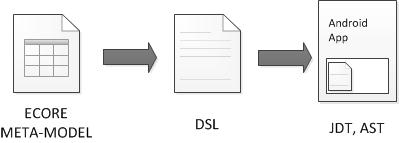
\includegraphics[width=0.8\textwidth]{flowchart}
  \caption{Flow chart}
\end{figure}

We started our project by determining the meta-model of the Android Intents. We based our model on several examples taken from Open Intents website\footnote{http://www.openintents.org/en/} and the knowledge presented in the chapter \ref{intents}. We show our ECore meta-model in the figure \ref{meta-model}.

\begin{figure}[H]
\label{meta-model}
  \centering
    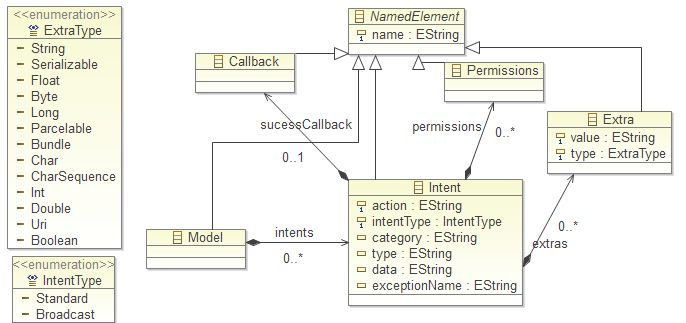
\includegraphics[width=\textwidth]{metamodel}
  \caption{Meta-model of Intent}
\end{figure}

Next we created grammar for our DSL by using XText and we made some examples of Intents in DSL to proof that the model based on is working. We use these newly created Intents as a database for our plug-in. The example of an Intent in our DSL is shown below:

{\footnotesize\begin{lstlisting}
ImplicitIntent ActionSendText {
	type "text/plain"
	category "android.intent.category.DEFAULT"
	action "android.intent.action.SEND"
	extras {
		StringExtra "android.intent.extra.TEXT" 
		"Put your text here"
	}
},
\end{lstlisting}}

Later we develop the Eclipse plug-in. For this purpose we use JDT and AST explained in the chapter \ref{tools}. JDT is used to modify Java source code and AST is used to access Java source code. We load our abstract syntax of Android Intents and we transform it into Abstract Syntax Tree, which is a simple Model To Model Transformation (M2M).

Our plug-in view is presented in the figure \ref{codegeneratorview}. An user can choose an intent and double-click on it. The generated code stub will appear on the place where the cursor is. If the cursor is positioned outside the method, it will create the method with the intent code inside. It is also possible to search for a specific intent in our intents database and to turn on or off the exception handling.

\begin{figure}[H]
\label{codegeneratorview}
  \centering
    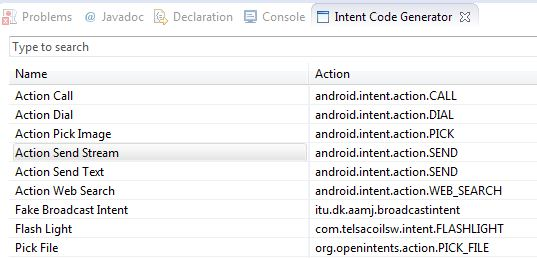
\includegraphics[width=\textwidth]{codegenerator}
  \caption{Code generator view}
\end{figure}

We present the generated code below for an Intent which sends a customized text to a non specified receiver.

{\footnotesize\begin{lstlisting}
public class IntentExample
{
	private string text = "Hello World";
	int sendText(){
		Intent ast = new Intent("android.intent.action.SEND");
		ast.setType("text/plain");
		ast.putExtra("android.intent.extra.TEXT", text);
		startActivity(ast);		
	}
}
\end{lstlisting}}